\documentclass[11pt,onecolumn]{article}
\usepackage[margin=1in]{geometry}
\usepackage{setspace}
\singlespacing
\usepackage{amsmath,amssymb}
\usepackage{graphicx}
\usepackage{booktabs}
\usepackage[hidelinks]{hyperref}
\usepackage{microtype}
\usepackage{hyperref}
\setlength{\parindent}{0.25in}
\setlength{\parskip}{0pt}

\title{\textbf{The Effect of Learning Rates on Gradient Descent Convergence: A Computational Study Using Linear Regression}}
\author{Miriam Abbate\\
Department of Mathematics, University of Tennessee, Knoxville\\
\texttt{mabbate3@vols.utk.edu}}
\date{}

\begin{document}
\maketitle

\begin{abstract}
This study investigates how the learning rate affects the convergence speed and stability of gradient descent for a simple linear regression problem. A synthetic dataset of 100 observations was generated from a linear model with Gaussian noise, and gradient descent was implemented to minimize the mean squared error. Three learning rates were selected as $0.05/L$, $0.5/L$, and $1.0/L$, where $L$ is the largest eigenvalue of the objective's Hessian. All experiments used the same data, zero initialization, and 300-update budget. The ordinary least-squares solution served as a reference, and convergence was defined by an objective gap below $10^{-6}$. The small, moderate, and large learning rates reached this tolerance after 200, 17, and 6 parameter updates, respectively. Each configuration approached the same minimum objective, approximately 0.11045406, and none diverged. Thus, for this particular quadratic problem, the largest tested learning rate converged fastest while remaining stable. The result illustrates that learning-rate choice can substantially affect optimization speed, while also emphasizing that a larger step is beneficial only when it remains within a suitable stability range.
\end{abstract}

\noindent\textbf{Keywords:} Gradient descent, learning rate, linear regression, optimization, convergence, machine learning.

\section{Introduction}
Machine learning often requires estimating model parameters by minimizing an objective function. Gradient descent is a basic optimization method that repeatedly adjusts parameters in the direction opposite the gradient. Its simplicity makes it useful across machine-learning applications, but its behavior depends strongly on the learning rate, or step size. A small step can make progress slowly; a step that is too large can overshoot a minimum and cause oscillation or divergence. Numerical optimization is therefore an important part of practical machine learning, as discussed by Bottou, Curtis, and Nocedal~\cite{bottou2018}.

This project asks: \emph{How does the choice of learning rate affect the convergence speed and stability of gradient descent when solving a linear regression problem?} To answer this question, we compare three learning rates on one reproducible synthetic dataset while holding the initialization, objective, and update budget fixed. This project uses a simple experiment to show how the shape of the least-squares objective affects how quickly gradient descent converges.

\section{Methodology}
\subsection{Model and objective}
For observation $i$, the prediction is
\[
\hat y_i=w_0+w_1x_i,
\]
where $w_0$ is the intercept and $w_1$ is the slope. Let $\theta=[w_0,w_1]^T$, let $X$ contain a column of ones and the input values, and let $y$ be the vector of observed responses. Then $\hat y=X\theta$. The parameters are chosen to minimize the half-scaled mean squared error
\[
J(\theta)=\frac{1}{2n}\|X\theta-y\|_2^2,
\qquad
\theta^*=\arg\min_{\theta}J(\theta).
\]
The factor $1/2$ is included to simplify differentiation. Differentiating with respect to the parameter vector gives
\[
\nabla J(\theta)=\frac{1}{n}X^T(X\theta-y).
\]
In component form, the two derivatives are $n^{-1}\sum_i(\hat y_i-y_i)$ and $n^{-1}\sum_i(\hat y_i-y_i)x_i$. They measure how the objective changes as the intercept and slope change.

\subsection{Gradient descent and learning rates}
Gradient descent uses all observations to calculate each update:
\[
\theta_{t+1}=\theta_t-\alpha\nabla J(\theta_t),
\]
where $\alpha$ is the learning rate. The Hessian of this quadratic objective is $H=X^TX/n$. Let $L$ be its largest eigenvalue. For this full-rank quadratic problem, the step-size condition $0<\alpha<2/L$ is sufficient for convergence \cite{chong2023optimization}. We used three rates, $0.05/L$, $0.5/L$, and $1.0/L$, which were approximately 0.0477, 0.4768, and 0.9536. Each is inside the stated stability interval.

Parameters were initialized at $\theta_0=[0,0]^T$. Each run performed 300 parameter updates. The reference optimum $\theta^*$ and its objective value were computed with NumPy's least-squares solver. Convergence speed was measured as the first update $t$ for which
\[
J(\theta_t)-J(\theta^*)<10^{-6}.
\]
The implementation used NumPy for numerical computation and Matplotlib for the convergence plot~\cite{harris2020,hunter2007}. The synthetic observations and the random seed are specified below so the experiment can be reproduced.

\subsection{Data generation}
The dataset contains $n=100$ observations generated according to
\[
y_i=3+2x_i+\epsilon_i,
\]
where each $x_i$ was sampled independently from a standard normal distribution and each noise term $\epsilon_i$ was sampled independently from a normal distribution with mean zero and standard deviation 0.5. The random seed was set to 42. 

\section{Experimental Results}
The least-squares reference estimates were an intercept of 3.003714 and a slope of 1.928371, with minimum objective $J(\theta^*)=0.11045406$. Table~\ref{tab:final} reports the parameter estimates after the full 300 iterations. The smallest learning rate remained slightly farther from the reference parameters, although its objective matched the others to the displayed precision.

\begin{table}[htbp]
\centering
\caption{Final parameter estimates after 300 updates.}
\label{tab:final}
\begin{tabular}{lrrr}
\toprule
Learning rate & Intercept & Slope & Final objective\\
\midrule
0.0477 & 3.003698 & 1.928339 & 0.11045406\\
0.4768 & 3.003714 & 1.928371 & 0.11045406\\
0.9536 & 3.003714 & 1.928371 & 0.11045406\\
\bottomrule
\end{tabular}
\end{table}

The number of parameter updates required to reach the objective-gap tolerance differed substantially. The small learning rate required 200 updates, the moderate rate required 17, and the large rate required 6. Thus, the moderate rate used about 11.8 times fewer updates than the small rate, and the large rate used about 33.3 times fewer. 

Figure~\ref{fig:convergence} plots the objective gap over the optimization trajectory. The small step decreases the gap gradually, while the moderate and large steps reduce it much more quickly. The large step is fastest among the tested values and shows no divergence or sustained oscillation. This is consistent with the fact that all three learning rates satisfy the quadratic stability condition. The result does not imply that increasing the learning rate always improves convergence: a rate outside an appropriate range can make gradient descent unstable.

\begin{figure}[h]
\centering
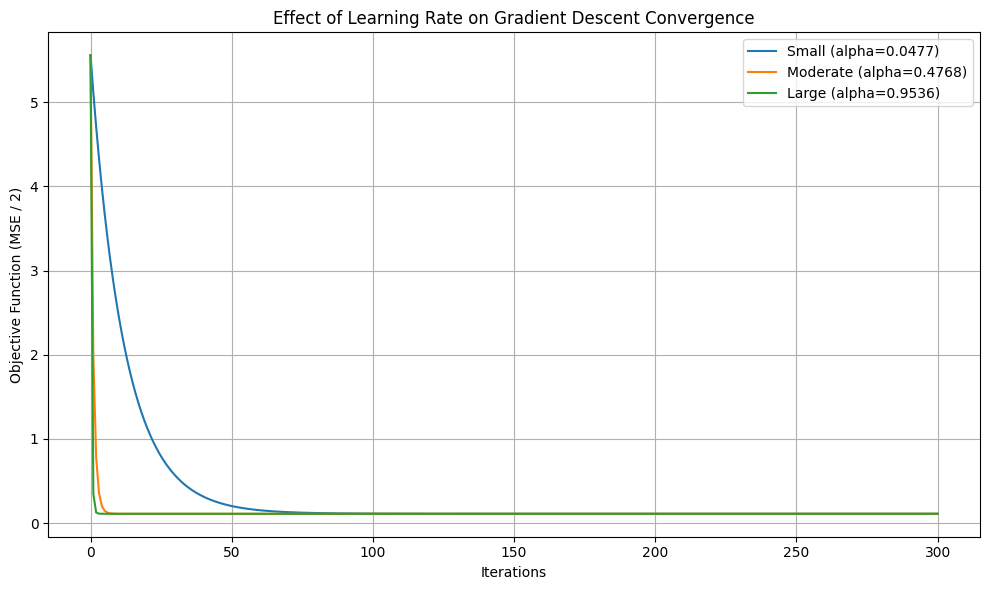
\includegraphics[width=0.82\linewidth]{convergence_plot.png}
\caption{Objective gap $J(\theta_t)-J(\theta^*)$ versus the number of gradient-descent parameter updates.}
\label{fig:convergence}
\end{figure}

This experiment has several limitations. It uses one synthetic dataset, one input feature, and three learning rates. It therefore does not establish how the same rates would behave on more complex or higher-dimensional problems. In addition, the comparison concerns optimization of the fixed training objective rather than generalization to new observations. Further work could repeat the experiment over multiple random seeds, test more learning rates, and compare gradient descent with momentum or adaptive optimization methods.

\section{Conclusion}
This study examined how learning-rate choice affects gradient descent for a simple linear regression objective. The largest tested rate, 0.9536, reached the objective-gap tolerance in 6 updates, compared with 17 updates for 0.4768 and 200 for 0.0477. All three runs approached the same least-squares minimum, and none diverged. For this dataset and quadratic objective, the largest tested rate was therefore the most efficient in iteration count while remaining stable. The main lesson is that learning rate has a substantial effect on convergence speed, but it must be chosen with the objective's curvature and stability range in mind. The small scope of the experiment limits generalization; multiple datasets, features, and optimization methods are natural next steps.

\section*{Code Availability}
The experiment code will be available at

\url{https://github.com/orso-99/csds513-learning-rate-gradient-descent}. 

\section*{Acknowledgment of AI Assistance}
Generative AI assistance was used to help organize and edit the LaTeX report and to prepare reproducibility materials. The author is responsible for reviewing the mathematical explanations, verifying the implementation and reported results, and approving the final submission.

\begin{thebibliography}{9}
\bibitem{bottou2018}
L. Bottou, F. E. Curtis, and J. Nocedal, ``Optimization Methods for Large-Scale Machine Learning,'' \textit{SIAM Review}, vol. 60, no. 2, pp. 223--311, 2018, doi: 10.1137/16M1080173.

\bibitem{chong2023optimization}
E. K. P. Chong, W.-S. Lu, and S. H. Zak,
\textit{An Introduction to Optimization: With Applications to Machine Learning},
5th ed. Wiley, 2023.

\bibitem{harris2020}
C. R. Harris et al., ``Array programming with NumPy,'' \textit{Nature}, vol. 585, pp. 357--362, 2020, doi: 10.1038/s41586-020-2649-2.

\bibitem{hunter2007}
J. D. Hunter, ``Matplotlib: A 2D Graphics Environment,'' \textit{Computing in Science \& Engineering}, vol. 9, no. 3, pp. 90--95, 2007, doi: 10.1109/MCSE.2007.55.
\end{thebibliography}

\end{document}